{
\usebackgroundtemplate{\tikz\node[opacity=0.07,inner sep=0] {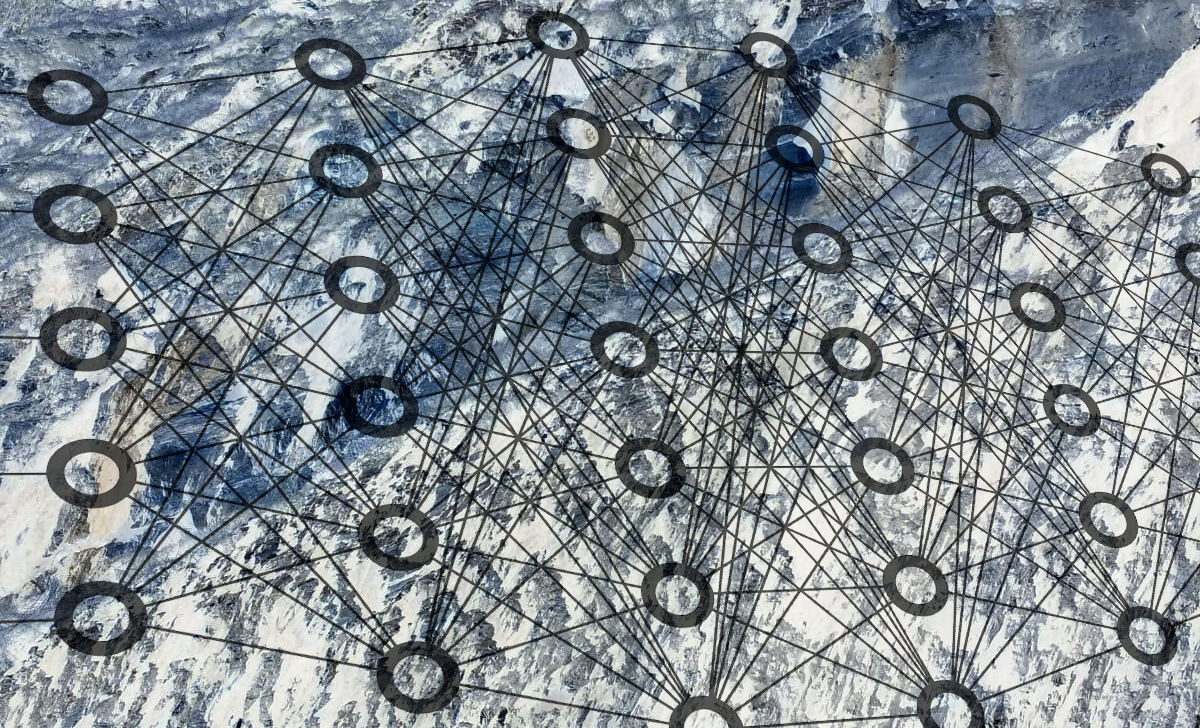
\includegraphics[height=\paperheight,width=\paperwidth]{frames/auxiliar/title_img/prueba.png}};}

\begin{frame}{Outline}
\begin{columns}
\begin{column}{0.05\textwidth}
\end{column}
\begin{column}{0.95\textwidth}

\mybullet{1}{Goal-Oriented $hp$-adaptivity for non-parametric PDEs}
	\vspace{-0.2cm}
	\begin{itemize}\setlength{\itemindent}{1cm}
	\item Why \( hp \)-Adaptivity?
	\item Goal-Oriented coarsening strategy      
	\item 1D Numerical results for Goal-Oriented $h$- and $p$-adaptivity
	\item 2D Numerical results for $hp$-adaptivity
	\item 3D Numerical results for $hp$-adaptivity
	\end{itemize}

\vspace{0.4cm}

\mybullet{2}{Goal-Oriented $hp$-adaptivity for parametric PDEs.}
	\vspace{-0.2cm}
	\begin{itemize}\setlength{\itemindent}{1cm}
	\item Database generation for DL inversion
	\end{itemize}

\vspace{0.4cm}

\mybullet{3}{Main Achievements}

\vspace{0.4cm}

\mybullet{4}{Conclusions and Future Work}
\end{column}
\end{columns}

\end{frame} 
}